\documentclass[11pt,a4paper]{article}
\usepackage[utf8]{inputenc}
\usepackage[margin=1in]{geometry}
\usepackage{graphicx}
\usepackage{booktabs}
\usepackage{hyperref}
\usepackage{listings}
\usepackage{xcolor}
\usepackage{tikz}
\usetikzlibrary{shapes.geometric, arrows, positioning, fit, backgrounds}

\definecolor{codegreen}{rgb}{0,0.6,0}
\definecolor{codegray}{rgb}{0.5,0.5,0.5}
\definecolor{codepurple}{rgb}{0.58,0,0.82}
\definecolor{backcolour}{rgb}{0.95,0.95,0.92}

\lstdefinestyle{mystyle}{
    backgroundcolor=\color{backcolour},   
    commentstyle=\color{codegreen},
    keywordstyle=\color{magenta},
    numberstyle=\tiny\color{codegray},
    stringstyle=\color{codepurple},
    basicstyle=\ttfamily\footnotesize,
    breakatwhitespace=false,         
    breaklines=true,                 
    captionpos=b,                    
    keepspaces=true,                 
    showspaces=false,                
    showstringspaces=false,
    showtabs=false,                  
    tabsize=2
}
\lstset{style=mystyle}

\title{\textbf{Stage 3 Voice Agent Upgrade Report}\\[0.5em]
\large JSON-Driven Flow Engine with Voice Activity Detection}
\author{Victor Ibhafidon}
\date{January 29, 2026}

\begin{document}

\maketitle

\section{Executive Summary}

In this report, I detail the Stage 3 upgrade to the Fortell Voice Agent system, introducing a \textbf{Retell AI-style architecture} with JSON-driven conversation flows and Voice Activity Detection (VAD). This upgrade addresses critical user experience issues while maintaining a lightweight infrastructure.

\subsection{Key Improvements}
\begin{itemize}
    \item \textbf{Fixed "Bot Responds Too Fast"}: Replaced fixed 1.5-second audio buffer with intelligent VAD-based speech detection
    \item \textbf{No-Code Flow Customization}: Conversation flows now defined in JSON files—no code deployment needed
    \item \textbf{Enhanced State Management}: Dynamic variable extraction with equation and LLM-based transitions
\end{itemize}

\section{Technical Implementation}

\subsection{Problem Statement}

The previous implementation (Stage 1/2) had two critical issues:

\begin{enumerate}
    \item \textbf{Premature Response}: The bot processed audio every 1.5 seconds regardless of whether the user finished speaking, causing interruptions mid-sentence.
    \item \textbf{Hardcoded Flows}: Any conversation flow change required Python code modifications and redeployment.
\end{enumerate}

\subsection{Solution: Voice Activity Detection (VAD)}

\begin{table}[h]
\centering
\begin{tabular}{@{}lll@{}}
\toprule
\textbf{Aspect} & \textbf{Before (Stage 1/2)} & \textbf{After (Stage 3)} \\
\midrule
Speech Detection & Fixed 1.5s buffer & Silero VAD model \\
End-of-Speech & Time-based & 600ms silence threshold \\
Interruption & Not supported & Barge-in enabled \\
Processing & Every 1.5 seconds & Only when speech complete \\
\bottomrule
\end{tabular}
\caption{VAD Implementation Comparison}
\end{table}

\subsection{Solution: JSON-Driven Flow Engine}

Conversation flows are now defined in JSON with the following structure:

\begin{lstlisting}[language=json, caption=Sample Flow Node Definition]
{
  "id": "collect_date",
  "type": "conversation",
  "instruction": "Ask for appointment date",
  "extract_variables": ["date"],
  "edges": [
    {
      "target_node_id": "collect_time",
      "conditions": [
        {"type": "equation", "condition": "{{date}} exists"}
      ]
    }
  ]
}
\end{lstlisting}

\textbf{Supported Node Types:}
\begin{itemize}
    \item \texttt{conversation} — Dialogue with user, variable extraction
    \item \texttt{function} — Execute API calls (calendar, external services)
    \item \texttt{logic\_split} — Conditional branching
    \item \texttt{end} — Terminate conversation
    \item \texttt{transfer} — Handoff to human agent
\end{itemize}

\section{Enterprise Architecture Comparison}

I evaluated the infrastructure required to match enterprise providers like Retell AI:

\subsection{Retell-Scale Architecture}

\begin{center}
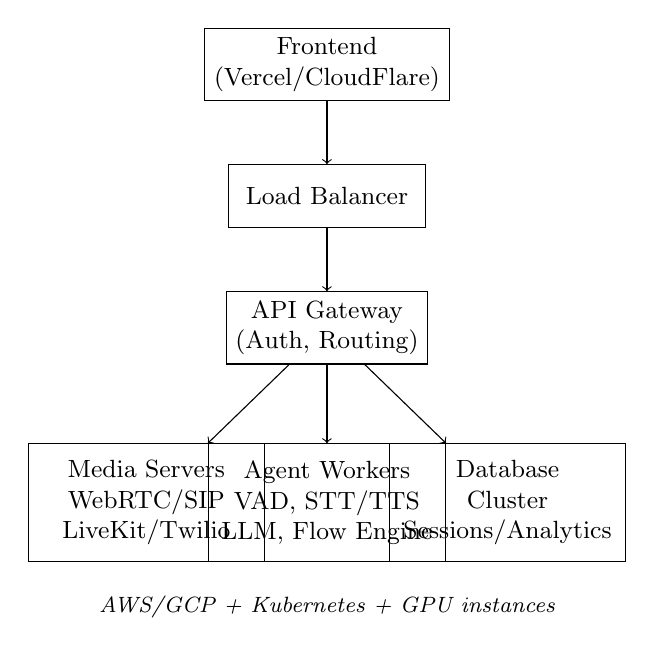
\begin{tikzpicture}[
    node distance=0.8cm,
    box/.style={rectangle, draw, minimum width=2.5cm, minimum height=0.8cm, align=center, font=\small},
    bigbox/.style={rectangle, draw, minimum width=3cm, minimum height=1.5cm, align=center, font=\small},
    every node/.style={font=\small}
]

% Top layer
\node[box] (frontend) {Frontend\\(Vercel/CloudFlare)};
\node[box, below=of frontend] (lb) {Load Balancer};
\node[box, below=of lb] (api) {API Gateway\\(Auth, Routing)};

% Bottom layer - three boxes
\node[bigbox, below left=1cm and -0.5cm of api] (media) {Media Servers\\WebRTC/SIP\\LiveKit/Twilio};
\node[bigbox, below=1cm of api] (agents) {Agent Workers\\VAD, STT/TTS\\LLM, Flow Engine};
\node[bigbox, below right=1cm and -0.5cm of api] (db) {Database\\Cluster\\Sessions/Analytics};

% Arrows
\draw[->] (frontend) -- (lb);
\draw[->] (lb) -- (api);
\draw[->] (api) -- (media);
\draw[->] (api) -- (agents);
\draw[->] (api) -- (db);

% Label
\node[below=0.3cm of agents, font=\footnotesize\itshape] {AWS/GCP + Kubernetes + GPU instances};

\end{tikzpicture}
\end{center}

\subsection{Infrastructure Tradeoff Analysis}

\begin{table}[h]
\centering
\begin{tabular}{@{}p{3cm}p{5cm}p{5cm}@{}}
\toprule
\textbf{Requirement} & \textbf{Retell-Scale (Enterprise)} & \textbf{My Approach (Stage 3)} \\
\midrule
Media Servers & Dedicated WebRTC/SIP infrastructure, multi-region & LiveKit Cloud (managed) \\
\addlinespace
Compute & Kubernetes clusters, GPU instances for inference & LiveKit Cloud workers \\
\addlinespace
Scaling & Auto-scaling to 10,000+ concurrent calls & Hundreds of concurrent calls \\
\addlinespace
Cost & \$10,000+/month base infrastructure & Pay-per-minute (\$0.01-0.05/min) \\
\addlinespace
DevOps & Dedicated team required & Minimal overhead \\
\addlinespace
Time to Deploy & 2-4 weeks initial setup & Same day \\
\bottomrule
\end{tabular}
\caption{Infrastructure Comparison}
\end{table}

\section{Decision: Current Infrastructure}

\subsection{Why I Chose to Stay Lightweight}

After evaluating enterprise-scale options, I decided to maintain the current infrastructure for the following reasons:

\begin{enumerate}
    \item \textbf{Cost Efficiency}: Enterprise infrastructure requires \$10,000+/month base cost. My LiveKit Cloud approach costs only per actual usage (\$0.01-0.05 per minute).
    
    \item \textbf{Operational Simplicity}: Kubernetes clusters, GPU instances, and multi-region deployments require dedicated DevOps expertise. My current setup requires minimal maintenance.
    
    \item \textbf{Sufficient Scale}: LiveKit Cloud can handle hundreds of concurrent conversations—adequate for current and near-term projected load.
    
    \item \textbf{Feature Parity}: Stage 3 delivers the core Retell-style features (JSON flows, VAD, dynamic variables) without the infrastructure complexity.
\end{enumerate}

\subsection{When to Reconsider}

I recommend revisiting infrastructure decisions when:
\begin{itemize}
    \item Concurrent call volume exceeds 500+ regularly
    \item LiveKit Cloud costs exceed \$5,000/month
    \item SIP/telephony integration becomes required
    \item Custom media routing is needed
\end{itemize}

\section{Files Delivered}

\begin{table}[h]
\centering
\begin{tabular}{@{}ll@{}}
\toprule
\textbf{File} & \textbf{Purpose} \\
\midrule
\texttt{backend/agent/flow\_engine/} & Complete flow engine module \\
\texttt{backend/flows/appointment\_booking.json} & Sample appointment flow \\
\texttt{backend/main\_stage3.py} & Stage 3 entry point \\
\texttt{docs/STAGE3\_FLOW\_ENGINE.md} & Technical documentation \\
\bottomrule
\end{tabular}
\caption{New Files}
\end{table}

\section{Activation}

To enable Stage 3, set in \texttt{.env}:

\begin{lstlisting}[language=bash]
AGENT_STAGE=stage3
VAD_ENABLED=true
VAD_SILENCE_THRESHOLD_MS=600
\end{lstlisting}

\section{Conclusion}

I designed Stage 3 to deliver enterprise-grade conversation flow capabilities while maintaining a lean infrastructure approach. The JSON-driven architecture enables rapid iteration on conversation design without engineering deployment cycles, and VAD significantly improves user experience by eliminating premature bot responses.

\textbf{Recommended Next Steps:}
\begin{enumerate}
    \item Test Stage 3 in development environment
    \item Fine-tune VAD thresholds for production audio quality
    \item Customize conversation flows for specific use cases
    \item Monitor performance metrics after deployment
\end{enumerate}

\end{document}
